\chapter{Designing Software for The Fast Multipole Method}\label{chpt:designing_software_for_fmm}
\thispagestyle{chaptertitle} % Force the fancy style on this page


\section{Data Oriented Design with Rust Traits}

- Motivation, and review, DOD book.

- How do traits enable data oriented design.

- Overview of the design of the software.

- Diagram for principal traits and how they link together in the final software.

- Why is this good for the future? Well, it leaves open extension to other approaches for any individual subcomponent.

- An example of this is the genericity over data type, kernel implementation, and field translation method, with a space for the kind of tree data structure.

\section{FMM Software As A Framework}

- Want to encourage as much code re-use as possible.

- The re-implementation of critical subcomponents should be avoided. A step towards this is the development low-level C interfaces which enable the construction of higher level interfaces in compatible languages.

- We've made a start to this with a low-level interface to the principal API of the FMM software.


- We also want to be able to deploy on as wide a range of target hardware as possible, and leave open extension to future systems, enabled by design, referencing diagram.

- High level diagram of how software components fit together

- Explain the diagrams (will need zoomed in diagrams for things like M2L data)

- Decouple implementation from

- Code generation for multiple targets enabled by Rust's llvm based compiler.

- C ABI as a compatiblity layer to other projects, success with this in developing Python wrappers and integration with NGBEM

- Flexible backends enabled by RLST package for BLAS and Lapack.


\section{High Performance Trees}

- Exactly how are Morton encodings done, and what are the drawbacks and alternatives.

- ORB (how does it work)

- Tree Construction approach and algorithms
    - Morton encoding via lookup tables
    - neighbour finding
    - interaction list construction (fast)

- What did we end up doing, and what is the justification for these being good enough.


Important implementation details
    - construction of interaction lists, neighbour finding.
    - construction of Morton encodings.
    - trade-offs of approach in shared and distributed memory
        - e.g. adaptive vs weakly adaptive trees.
        - problems with load balancing approach etc
    - justification
        - simplicity/works vs complex/private


\section{High Performance FMM Operators}

- FMM data flow, mapping its tree structure to a data flow diagram.

- Go through each operator of kiFMM and how it's been optimised, at a high level for M2L operators.

\subsection{Point to Multipole (P2M)}

- Formulation in a blocked manner
\subsection{Multipole to Multipole (M2M) and Local to Local (L2L)}

- Formulation as BLAS3

\subsection{Point to Point (P2P)}

- Computational challenge (SIMD/SIMD), and why this is the easiest to optimise.

\subsection{Multipole to Local (M2L)}

- Description of computational challenge due to memory layout proscribed by Morton encoding.

- Formulation of the problem, and required precomputations.

- Data structure required to be flexible over this.


How future FMMs may look, shallow trees with large P2P.



% \section{Performance Model}


% \section{Distributed FMM}

% \section{Helmholtz FMM}


% Q. What is the FMM, and how does it fit into an ecosystem of Fast Algorithms?

    - Introduce the algorithmic intuition for the FMM very briefly.
        - Dump the algorithm in the appendix.
    - Zoo of FMMs/Hierarchical algorithms that have similar algorithm structure.
    - Utility relies on problem context.
        - Where some FMMs are preferable to others.
        - This makes a generic software hard \dots
    - Some FMMs are amenable to generic implementation that target a wide-class
    of problems, black box.
        - KiFMM
            - How does it create multipole and local expansions - MFS.
                - Dump MFS further explanation in the appendix.
            - How does it compute the translation operators?
                - turn it into a least squares problem
        - bbFMM
            - How does it create multipole and local expansions? Cheb.
            - How does it compute translation?
                - Not sure, need to check.

Q. What are the main challenges associated with developing bbFMMs?

    - Performant multipole to local translations. Which in bbFMMs are a matvec.
        - Main approaches to accelerate this are SVD and FFT.
        - How do these work, roughly?
            - Dump detailed explanation in the appendix.
        - Can count flops for different approaches
        - Implementation challenges
            - memory ordering for fft
            - fast ffts
            - blas3 for SVD
            - designing a generic interface for developers
            - fast trees, that can also work in dist memory
                - communication bottlenecks, and potential approaches

        - dump all algorithms into appendix

Q. What about other fast algorithms, do they require any of the same stuff used
in the FMM? What are the key areas to make generic as an implementer, has this
been done before?

    - Inverse FMM H matrix inverses, other fast direct solver approaches all
    rely on fast trees
    - trees are actually widely used in other sci comp tasks
        - current tree software, p4est
            - why can we not just use this?
                - want cross platform builds trivial
    - want to design a hierarchy of interfaces that can be used for our application,
    but also easily plug in to other work.



% \section{Algebraic FMM Variants}\label{chpt:2:sec:1}

In its original analytical form the applicability of the FMM is limited by the requirement for explicit multipole and local expansions, as well as a restriction to matrix vector products. Subsequent decades saw the development of `algebraic' analogues to the original algorithm. These methods are similarly based on a hierarchical partitioning, whether that be of the point data using a recursive tree as with the original FMM \cite{Ying:2004:JCP,fong2009black}, or by operating on the matrix implied by the FMM's algorithmic structure directly \cite{hackbusch1999sparse,borm2003introduction,chandrasekaran2007fast}. The latter methods are collectively known as $\mathcal{H}^2$-matrix methods. Representing the FMM operation in this way has allowed the extension of the FMM to other matrix computations, such as matrix-matrix products, as well as approximations of its inverse \cite{ambikasaran2014inverse}. Notably, many of these methods don't necessarily rely on explicit multipole/local expansions for approximating fields as in the original FMM in the previous section. Examples such as the `kernel independent FMM' (kiFMM) of Ying and co-authors instead relies on the method of fundamental solutions to approximate the fields and requires only evaluating kernel values, and is applicable to a wide range of kernels from second-order linear non-oscillatory elliptic PDEs with constant coefficients such as the Laplace equation. This approach relies on some analytic considerations, however methods also exist which are interpolatory - such as the `black box FMM' (bbFMM) of Fong and Darve \cite{fong2009black}, which similarly only relies on kernel evaluations and a Chebyshev scheme to approximate fields.

In our software we choose to implement the kiFMM of Ying and coauthors, which we explain in detail below adapting the discussion from Section 3 of \cite{Ying:2004:JCP}. This method shares advantages with other algebraic FMM methods, of generality to a large class of problems, as well as opportunities to optimise computer implementations we explore in Section \ref{chpt:2:sec:1}. This approach relies on a spatial discretisation of the problem domain via an quad/octree as in the original FMM, as well as the method of fundamental solutions (MFS) for approximating the fields from point charges/masses. This method has been demonstrated to perform well on shared memory systems \cite{wang2021exafmm}, achieve similar accuracy to the analytical variant, with relatively low pre-computation required\footnote{This depends heavily on the choice of how to sparsify $T^{M2L}$, see Section \ref{chpt:3:sec:1:m2l} for more details.}. The underlying data structure of the quad/octree has been a significant area of research and development, with established high-performance methods for their construction in shared/distributed memory environments \cite{sundar2008bottom,sundar2013hyksort,BursteddeWilcoxGhattas11}.

Consider the kernels for second-order constant coefficient non-oscillatory PDEs, such as that of the Laplace equation in (\ref{eq:chpt:2:sec:0:laplace_kernel}). Such kernels satisfy the underlying PDE everywhere except the singularity location, and are smooth away from this singularity. These problems admit a unique solution for interior/exterior Dirichlet boundary value problems. The authors of \cite{Ying:2004:JCP} rely on the smoothness and uniqueness of the Dirichlet boundary value problems as basic properties to develop their FMM formulation. The problem setting as before is the calculation of (\ref{eq:chpt:2:sec:0:fmm_problem}) for the Laplace kernel, for a set of $N$ point sources $y_i$, $i = 1...N$, which we will associated with $N$ source densities $q_i$, an target locations $y_j$, $j=1...M$. As before, the source and target locations may coincide. We use an index set $I^B_s$ and $I^B_t$ to identify the sources and targets we are considering in a particular interaction. We assume that our problem is in $\mathbb{R}^3$, however the exposition is essentially the same as in $\mathbb{R}^2$.

Assuming that we have constructed our hierarchical tree partitioning, which may be adaptive, the first step is to approximate the fields due to particles contained in each leaf box. We specify more concretely that for a given box, $B$, its `near field range', $\mathcal{N}^B$, is the set of 27 boxes at the same level of a tree which are adjacent to it, i.e. they share a corner, face or edge as well as $B$ itself. Its `far field range', $\mathcal{F}^B$, is simply the boxes which are the complement of this.

We approximate the potential in $\mathcal{F}^B$ from the source densities $\{ q_i : i \in B \}$ in $B$ using the potential from an \textit{equivalent density distribution}, $q^{B, u}$, supported at prescribed locations $y^{B, u}$ (see the left box in Figure \ref{fig:chpt:2:sec:1:multipole_local}). Where $q^{B, u}$ is called the \textit{upward equivalent density} and $y^{B, u}$ is called the \textit{upward equivalent surface}. This amounts to representing the potential with a `single layer' potential \cite{Kress2014},

\begin{flalign}\label{eq:chpt:2:sec:1:single_layer_potential}
    \phi(x) &:= \int_{y \in y^{B, u}} K(x, y)q^{B, u}(y) ds(y), \> \> x \in \mathbb{R}^3 \setminus y^{B, u}
\end{flalign}

To guarantee the smoothness of the potential produced by $q^{B, u}$ in the far-field, its support $y^{B,u}$ must not overlap with $\mathcal{F}^B$ due to the singularities in this integral from the kernel function when evaluated on the equivalent surface. Secondly, we note that the equivalent surface must enclose $B$ from the definition of the single layer potential \cite{Kress2014}. We see that the equivalent surface must be placed in between the box and the boundary of $\mathcal{F}^B$.

The potential induced by our equivalent densities and upward equivalent surface satisfies the Laplace equation. Therefore, due to the uniqueness of the exterior Dirichlet boundary value problem for this kernel (as well of kernels of a similar type), we reason that the potential calculated using (\ref{eq:chpt:2:sec:0:fmm_problem}) directly from the source particles must be equivalent to that calculated using (\ref{eq:chpt:2:sec:1:single_layer_potential}) in $\mathcal{F}^B$, or anywhere between $y^{B, u}$ and $\mathcal{F}^B$. Thus we place an intermediate surface called the \textit{upward check surface} between $\mathcal{F}^B$ and $y^{B, u}$, denoting it with $x^{B, u}$. The potential computed at this surface is called the \textit{upward check potential}, which we denote by $\phi^{B, u}$.

We write this as,

\begin{flalign}\label{eq:chpt:2:sec:1:multipole_appx}
    \int_{y^{B, u}} K(x, y) q^{B, u} dy = \sum_{i \in I^B_s} K(x, y_i)q_i = \phi^{B, u}(x)\> \>, \text{for any } x \in x^{B, u}
\end{flalign}

Solving for the equivalent densities is an equivalent method of approximating the far-field potential induced by the points in $B$. We identify this with a \textit{multipole expansion}. Now considering source densities which are not contained in a box $B$ (see right box of Figure \ref{fig:chpt:2:sec:1:multipole_local}) but in its $\mathcal{F}^B$, we can construct an equivalence for local expansions using a similar approach. To ensure the existence of the \textit{downward equivalent densities} $q^{B, d}$, the \textit{downward equivalent surface}, $y^{B, d}$, must be located between $B$ and $\mathcal{F}^B$ and the potentials generated by the source points are matched to those generated by the equivalent points on a \textit{downward check surface}, $x^{B, d}$ that encloses the box and is itself enclosed by $y^{B, d}$ in order to calculate a \textit{downward check potential} $\phi^{B, d}$.

\begin{flalign}\label{eq:chpt:2:sec:1:local_appx}
    \int_{y^{B, d}} K(x, y) q^{B, d} dy = \sum_{i \in I^{\mathcal{F}^B}_s} K(x, y_i)q_i = \phi^{B, d}(x) \> \> \text{for any } x \in x^{B, d}
\end{flalign}

In $\mathbb{R}^3$ the authors chose to represent the equivalent and check surfaces as cubes, with the equivalent/check points arranged regularly over the surfaces. We choose the same as it leads to implementation benefits when designing the field translation operators (see Section \ref{chpt:3:sec:1:subsec:2:fft} for how we take advantage of this).

\begin{figure}
    \centering
    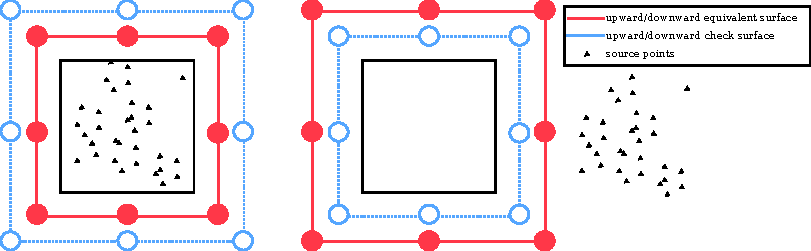
\includegraphics[width=\textwidth]{ch_2/p2m.pdf}
    \caption{ We illustrate the equivalent/check surfaces and associated boxes in $\mathbb{R}^3$, where we show a corresponding cross section. In the first figure, we illustrate the situation in the `P2M' operation, where we are trying to construct an approximation to the potential generated by points in a box by matching it to that generated by a set of equivalent density points placed on a fictitious surface enclosing it. In the second figure we illustrate the `P2L' operation, where we are now trying to construct an approximation to the  potential generated by points in a box's far-field within the box.}
    \label{fig:chpt:2:sec:1:multipole_local}
\end{figure}

Equations (\ref{eq:chpt:2:sec:1:multipole_appx}) and (\ref{eq:chpt:2:sec:1:local_appx}) are examples of \textit{Fredholm integral equations of the first kind}, the inversion of which is ill-posed. To solve these equations, we must first discretise, for which we made use of the \textit{Method of Fundamental Solutions} (MFS), a technique whereby the potential is approximated by a linear combination of kernel function evaluations at a set of discrete points with associated densities,

\begin{flalign}\label{eq:chpt:2:sec:1:mfs}
    \phi(x) \approx \phi^N(x) = \sum_{y_i \in y^{B, u}} K(x, y_i) q_i
\end{flalign}

Where $N$ denotes the number of equivalent points of density are placed on the equivalent surface. To see how this approximates the single-layer operator we used above to calculate the potential we simply replace the continuous density functions in (\ref{eq:chpt:2:sec:1:single_layer_potential}) with $\sum_{j=1}^N q_i \delta(y-y_j)$, recovering (\ref{eq:chpt:2:sec:1:mfs}). Writing (\ref{eq:chpt:2:sec:1:multipole_appx}) or (\ref{eq:chpt:2:sec:1:local_appx}) in matrix form reflecting the discretisation via MFS,

\begin{flalign}
    K q = \phi
\end{flalign}

We can solve the problem with Tikhonov regularisation,

\begin{flalign}
    q = (\alpha I + K^* K)^{-1}K^*\phi
\end{flalign}

which converts it into a matrix equation, that shares similarities in terms of well posedness with discretised \textit{Fredholm integral equations of the second kind}. The regularisation parameter $\alpha$ is found empirically. Computing (\ref{eq:chpt:2:sec:1:multipole_appx}) is equivalent to the $T^{P2M}$ operator described in the previous section for the analytical FMM, (\ref{eq:chpt:2:sec:1:local_appx}) is equivalent to an $T^{P2L}$ operator which was not explicitly described. As before, these operators take a set of charges, and create expansions that allow us to evaluate their potential in the far-field, however the method of creating the expansions is clearly significantly different. The most notable change being that our above formulation \textit{does not require explicit analytical expansions of the kernel function}, only making use of kernel evaluations.

To complete the kiFMM we need analogues to the field translation operators, $T^{M2L}$, $T^{M2M}$, $T^{L2L}$. We illustrate the required surfaces for each of these operators in Figure \ref{fig:chpt:2:sec:1:translations}. For $T^{M2M}$ we must translate the upward equivalent density of $A$ to the centre of its parent box $B$, solving the following equation for $q^{B, u}$,

\begin{flalign}
    \label{eq:chpt:2:sec:1:m2m}
    \int_{y^{B, u}} K(x, y)q^{B, u}(y)dy = \int_{y^{A, u}}K(x, y)q^{A, u}(y) dy, \> \> \text{for all } x \in x^{B, u}
\end{flalign}

As before, $y^{A, u}$ must enclose the child box $A$. During the downward pass, we must evaluate the downward equivalent density, corresponding to a local expansion, from the multipole expansions of non-adjacent boxes in $B$'s parent neighbour's children. We similarly write down for $T^{M2L}$,

\begin{flalign}
    \label{eq:chpt:2:sec:1:m2l}
    \int_{y^{B, d}} K(x, y)q^{B, d}(y)dy = \int_{y^{A, u}}K(x, y)q^{A, u}(y) dy, \> \> \text{for all } x \in x^{B, d}
\end{flalign}

Finally, the local expansions of each box $B$ must be translated to the centre of each of its children $A$,

\begin{flalign}
    \label{eq:chpt:2:sec:1:l2l}
    \int_{y^{B, d}} K(x, y)q^{B, d}(y)dy = \int_{y^{A, d}}K(x, y)q^{A, d}(y) dy, \> \> \text{for all } x \in x^{B, d}
\end{flalign}

For each of these translation operators we use the discretisation based on MFS discussed above, and solve using Tikhonov regularisation. For the  $T^{L2P}$, $P2P$ and $T^{M2P}$ operators we simply use direct kernel evaluations at the target points with respect to the equivalent densities represented by the multipole or local expansion coefficients or the true densities at the source points.

\begin{figure}
    \centering
    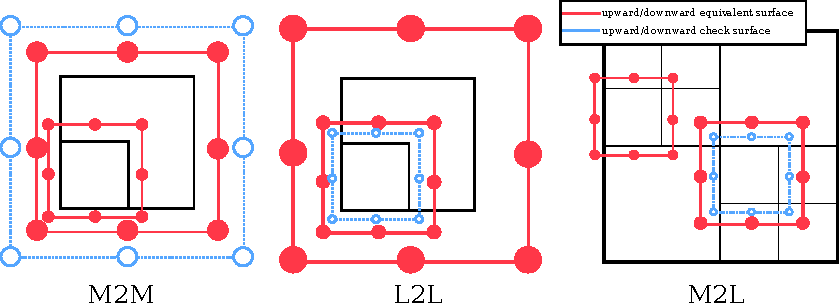
\includegraphics[width=\textwidth]{ch_2/translations.pdf}
    \caption{ As in Figure \ref{fig:chpt:2:sec:1:multipole_local}, we illustrate the translations as cross sections of the surfaces, which are cubes in $\mathbb{R}^3$.}
    \label{fig:chpt:2:sec:1:translations}
\end{figure}


% \section{Implementation Challenges for the Kernel Independent Fast Multipole Method }\label{chpt:2:sec:2}

In this section we introduce analytical features of the kernels compatible with the kiFMM that have consequences for computer implementations, such as the ability to pre-compute and cache matrices that correspond to translation operators. We also discuss the octree data structure in more detail, highlighting its key bottlenecks, concluding with a discussion on implied computational and storage complexity.

The defining feature of the kernels compatible with the FMM is that they they display a rapid decay behaviour as the distance between interactions increases, known formally as \textit{asymptotic smoothness}. A kernel is described as asymptotically smooth if there are constants $C_{\text{as1}}, C_{\text{as2}} \in \mathbb{R}_{>0}$ that satisfy \cite{borm2003introduction},

\begin{flalign}
        \label{eq:chpt:2:sec:1:asym_smooth}
    | \partial_x^\alpha \partial_y^\beta K(x, y) | \leq C_{\text{as1}} (C_{\text{as2}} \|| x-y \|_2)^{-|a|-|b|}\alpha + \beta|K(x, y)|
\end{flalign}

for all multi-indices $\alpha, \beta \in \mathbb{N}^3_0$ and all $x, y \in \mathbb{R}^3$. It's this smoothness that allows us to limit the definition of $\mathcal{N}^B$ to its neighbouring boxes in the FMM. Considering the situation in $\mathbb{R}^3$ only, this leads to $|\mathcal{N}^B| = 3^3=27$.

Far-field interactions are handled by the $T^{M2L}$ step, we saw above how this is limited to interactions with boxes which are children of $B$'s parent, but non-adjacent to $B$. Therefore we see that in a multi-level scheme the $\mathcal{N}^B$ contains all of the $6^3=216$ near and far field interactions of $B$'s children. As far-field interactions necessarily exclude the near field, this leads to a maximum of $6^3-3^3=189$ boxes in each child box's far field that must be considered, each corresponding to a single $T^{M2L}$. This is one of the \textit{key bottlenecks} of efficient FMM implementations. There are numerous ways of \textit{sparsifying} this step, either by using some additional numerical technique such as an SVD to compress the matrices corresponding to $T^{M2L}$ as they are known to be low-rank, or by using an exact method such as an Fast Fourier Transform (FFT) - which relies on our decision to place the equivalent densities on a regular grid as then the $T^{M2L}$ can be re-interpreted as a convolution. We discuss the trade-offs of these approaches in detail in Section \ref{chpt:3:sec:1:m2l}, as optimal implementations of this sparsification are of central importance to our software's performance.

We note that precomputations can be further reduced if kernels also exhibit translational invariance,

\begin{flalign}
    \label{eq:chpt:2:sec:1:translational_invariance}
    K(x, y) = K(x+v, y+v)
\end{flalign}

where $v \in \mathbb{R}^3$, we can compute $T^{M2L}$ for a restricted subset of the total possible interactions for the eight child boxes. Indeed, the union of all possible far-field interactions for the eight child boxes gives $7^3-3^3 = 316$ possible interactions. This comes from the fact some subset of translation vectors are non-overlapping for each child, resulting in a total of $7^3$ total interactions for all children, subtracting the near-field interactions which are the same for all children gives the result. Furthermore this means that we must pre-compute just 316 unique $T^{M2L}$ if our kernel has these favourable properties. This is of course dependent on choosing the same equivalent and check surfaces, and density locations, for each box. If so, these can be pre-computed and cached for a given expansion order, corresponding to all possible $T^{M2L}$ at each level.

If an asymptotically smooth, translationally invariant, kernel is also homogeneous to degree $n$,

\begin{flalign}
    K(\alpha r) = \alpha^n K(r)
\end{flalign}

where $\alpha \in \mathbb{R}$, implies that when we scale the distance between a source and target box by $\alpha$ the potential is scaled by a factor of $\alpha^n$, where $n$ depends on the kernel function in question, we can compute $T^{M2L}$ for a \textit{single} level of the tree, and scale the result at subsequent levels. This is summarised in Table \ref{table:chpt:2:sec:1:m2l_optimisations}.

\begin{table}
    \centering
    \caption{Number of near and far field boxes for a given box $B$, depending on the type of kernel we're considering.}
    \begin{tabular}{l l l}
        \toprule
        Kernel Type & boxes in $\mathcal{N}^B$ & boxes in $\mathcal{F}^B$ \\
        \midrule
        trans. invar. & $\leq$ 27 per box & $\leq$ 316 per level \\
        trans. invar. + homog. & $\leq$ 27 per box & $\leq$ 316 in total\\
        \bottomrule
    \end{tabular}
    \label{table:chpt:2:sec:1:m2l_optimisations}
\end{table}

As we've chosen the location of point densities to be fixed relative to each box, the evaluation of (\ref{eq:chpt:2:sec:1:m2m}) and (\ref{eq:chpt:2:sec:1:l2l}) can equivalently be pre-computed. In this case, there are just 8 unique matrices corresponding to $T^{M2M}$ and $T^{L2L}$, corresponding to the relative positions between a parent box and its children.

We observe the $T^{P2M}$ is calculated for all the nodes of a quad/octree in a discretisation, as observed in the previous section the level of discretisation is either specified by the user, or set by a user defined constraint $N_{\text{crit}}$ which specifies a maximum number of points contained within each leaf box. This leads to $O(N \cdot N_{\text{crit}})$ to find the check potentials for each leaf, therefore we note that $N_{\text{crit}}$ must be kept small to ensure linear complexity is maintained for this operation. To compute the equivalent density, we rely on an application of the inverted integral operator in (\ref{eq:chpt:2:sec:1:multipole_appx}). The size of this matrix is determined by the expansion order $P$, which determines the number of quadrature points taken on the equivalent/check surfaces. As the points are taken to be placed on a regular grid over this surface, the number of quadrature points $N_{\text{quad}}$ relates to $P$ as,

\begin{flalign}\label{eq:chpt:2:sec:2:ncoeffs}
    N_{\text{quad}} = 6(P-1)^2+2
\end{flalign}

Therefore, this matrix vector product is of $O((P-1)^4)$, leading to $O(N((P-1)^4 + N_{\text{crit}}))$ complexity for the entire operator. The complexity of $T^{P2L}$ is the same, as it amounts to the same calculation, albeit to form a local expansion. The precomputation of the translation operator requires an SVD for the integral operator in (\ref{eq:chpt:2:sec:1:multipole_appx}), the complexity of which is dependent on the algorithm chosen, with implementation specific optimisations. However, for a $\mathbb{R}^{m \times n}$ matrix where $m$ and $n$ are of similar size, the `DGESVD' implementation of LAPACK, which we use in our software framework, has a complexity of $O(n^3)$ therefore this precomputation is of $O((P-1)^6)$. The storage required is of $O((P-1)^4)$ for the inverted matrix.

Applying similar analysis for computing (\ref{eq:chpt:2:sec:1:m2m}) and (\ref{eq:chpt:2:sec:1:l2l}), we arrive at computational complexities of $O(N \cdot (P-1)^4)$ for calculating the check potentials, and then evaluating the equivalent densities via two matrix-vector products. For the M2L step, if we do not choose to implement any sparsification, we also obtain $O(N \cdot (P-1)^4)$ for the asymptotic complexity of applying $T^{M2L}$, however here there are large lurking constants. Specifically, each box $B$ has to apply an $T^{M2L}$ up to 189 times in $\mathbb{R}^3$ or 27 times in $\mathbb{R}^2$. The storage complexity is determined by the kernel, as shown by table \ref{table:chpt:2:sec:1:m2l_optimisations}, the properties of the kernel can reduce the number of precomputations that can be cached.

Similar large constants lurk in the leaf level computations $P2P$, $T^{M2P}$, $T^{P2L}$. These all consider boxes contained in $B$'s near field. For non-uniform point distribution there could be very large number of boxes contained in the near field. Therefore to reduce this we enforce a `balancing' condition, as mentioned above. The most common condition is a `2:1 balance', whereby neighbouring boxes are restricted to be no more than twice as large as each other \cite{malhotra2015pvfmm}. This restricts the size of the number of adjacent boxes to $B$ to be at most 52 in $\mathbb{R}^3$. For these boxes we will calculate the potential for points in $B$ using kernel evaluations directly via $P2P$. For the remainder of its near field, we'll use the $T^{M2P}$ operator. This operator considers boxes in $B$' near field for which the multipole expansion still applies at $B$, this means that leaf boxes that coincide with $B$'s neighbours children that are non-adjacent to $B$. At most there are 156 such boxes in $\mathbb{R}^3$. There may also be an additional contribution to the local expansion at $B$ not captured in $T^{L2L}$ and $T^{M2L}$, from boxes in the near-field of $B$'s parent which are the leaf level, and considered in the far-field of $B$ itself, and are the level of $B$'s parent. These contributions are found via $T^{P2L}$. With our balancing condition there are at most 19 such boxes in $\mathbb{R}^3$. We note that for uniformly refined trees $T^{M2P}$ and $T^{P2L}$ aren't calculated as their corresponding interactions are subsumed into $P2P$. The $P2P$ operator is therefore of $O(52 N \cdot N_{\text{crit}})$, with no storage cost as this is applied directly to points. Similarly, the complexity of $T^{M2P}$ is $O(156 N \cdot (P-1)^2 N_\text{crit})$, $T^{L2P}$ is of $O(N (P-1)^2 \cdot N_\text{crit})$. The complexity of $T^{P2L}$ is $O(19 N \cdot ((P-1)^4 + N_\text{crit}))$, where we include the cost of calculating the check potential as in $T^{P2M}$. The complexities of each step are summarised in table \ref{table:chpt:2:sec:2:kifmm_complexities}. These complexities are only an upper bound, for $T^{M2P}$ and $T^{P2L}$, and correspond to quite extreme point distributions, rarely occuring for all boxes in a given discretisation. In practice these are found to be an order of magnitude smaller than the number of boxes that must be considered in $T^{M2L}$ for point distributions that are relatively uniform \footnote{For example for randomly distributed on the surface of a sphere, or normally distributed points, typical values are $O(10)$ boxes for $T^{M2P}$ and $O(1)$ boxes for $T^{L2P}$}.

Therefore the largest bottlenecks are the $P2P$ and $T^{M2L}$ steps, and the area of focus in optimised implementations. When implemented naively, $T^{M2L}$ contains a large number of BLAS level 2 operations, and is calculated for every non-leaf box below the first level of an octree/quadtree. An obvious optimisation is to re-order data such that a single BLAS level 3 operation is computed for each box. This increases the ratio of computations to memory accesses by converting a series of matrix-vectors product into a single matrix-matrix product for each box. Additionally, the SVD taken for the integral operators above can be cut-off due to the low-rank nature of the above operators, leading to a reduced storage and application complexity. We explore the rank behaviour in more detail in Chapter \ref{chpt:3:sec:1:m2l} for the Laplace kernel. If instead one chooses to take an FFT, which offers lower complexity for each $T^{M2L}$ while being an exact translation, one has to compute the FFT corresponding to each unique translation which as we've seen is kernel dependent, and perform an inverse FFT to evaluate the check potentials at the equivalent density points. This leads to a lower overall complexity for both compute and storage - however, as we observe in Section \ref{chpt:3:sec:1:subsec:2:fft}, memory accesses are critical to performant implementations. The performance of the $P2P$, $T^{M2P}$ and $T^{L2P}$ operators are determined most significantly by the ability to rapidly evaluate the kernel function over sets of points. This is a ripe area for compute optimisations, such as GPU off-loading, or developing vectorised CPU code, and is therefore highly-dependent on the available computational resources and their respective architectures. Practical implementations should be flexible enough to for developers to `plug-in' different implementations in order to experiment with new hardware.

The second major bottleneck with the kiFMM and FMMs more generally, especially in a distributed setting, is the quad/octree data structure. The tree is crucial to performance as being able to rapidly query, and communicate via the tree, especially in a distributed setting will determine the overall runtime, as communication latency is a leading order variable in the distributed FMM's complexity \cite{Yokota2014}. Though there has been significant scholarship in developing high-performance tree libraries for parallel and distributed settings \cite{BursteddeWilcoxGhattas11,sundar2008bottom,sundar2013hyksort}, we observe that relatively little work has been done to examine and develop tree libraries with the FMM explicitly in mind, we explore potential optimisations in Section \ref{chpt:3:sec:0:octrees}. Specifically, $T^{M2M}$ summarises global information that is required by each box, and is later distributed via $T^{M2L}$ this necessarily involve communication across node boundaries in a distributed setting. Additionally, the broad applicability of parallel trees necessitates a design of software that is relatively de-coupled from the FMM code to encourage adoption in other communities. These two concerns determine the implementation strategy of our own tree library.

\begin{table}
    \centering
    \caption{Asmyptotic complexities of each kiFMM operator in $\mathbb{R}^3$, with constants left to demonstrate relative contrast. For $T^{M2L}$ we provide a few different complexity estimates, starting with `naive' implementation which applies the inverted integral equation (\ref{eq:chpt:2:sec:1:m2l}) up to 189 for each box as a matrix vector product, with no sparsification. Then the complexities with respect to different kernel properties. For an $T^{M2L}$ sparsified via the SVD we indicate a cut-off rank with $\kappa$, for an FFT based approach as we are often working with real data for the densities we can retain only half the calculated frequencies to save on storage costs. For the $T^{P2L}$, $T^{M2P}$ and $P2P$ operators we provide estimates for 2:1 balanced trees, as we restrict ourselves to this a practical implementation.}
    \begin{tabular}{l l l}
        \toprule
        Operator & Computational Complexity & Storage Complexity  \\
        \midrule
        $T^{P2M}$ & $O(N(36(P-1)^4 + N_{\text{crit}}))$ & $O(36(P-1)^4)$\\
        \midrule
        $T^{M2M}$ & $O(36N(P-1)^4)$ & $O(8 \cdot 36(P-1)^4)$\\
        \midrule
        $T^{L2L}$ & $O(36N(P-1)^4)$ & $O(8 \cdot 36(P-1)^4)$\\
        \midrule
        $T^{M2L}_\text{naive}$ & $O(189N \cdot 36(P-1)^4)$ & $O(189N \cdot 36(P-1)^4)$ \\
        \midrule
        $T^{M2L}_\text{trans. inv.}$ & $O(189N \cdot 36(P-1)^4)$ & $O(316 \log(N) \cdot 36(P-1)^4)$ \\
        \midrule
        $T^{M2L}_\text{homog+trans. inv.}$ & $O(189N \cdot 36(P-1)^4)$ & $O(316 \cdot 36(P-1)^4)$ \\
        \midrule
        $T^{M2L}_\text{homog+trans. inv. + SVD}$ & $O(189N \cdot 6(P-1)^2 \cdot \kappa )$ & $O(316 \cdot 6(P-1)^2 \cdot \kappa)$ \\
        \midrule
        $T^{M2L}_\text{homog+trans. inv. + FFT}$ & $O(189N \cdot 4 (P-1) \log(P-1))$ & $O(316 \cdot 36(P-1)^4)$ \\
        \midrule
    $T^{M2L}_\text{homog+trans. inv. + Real FFT}$ & $O(189 N \cdot 4 (P-1) \log(P-1))$ & $O(316 \cdot 18(P-1)^4)$ \\
        \midrule
        $T^{L2P}$ & $O(N(36(P-1)^4 + N_{\text{crit}}))$ & $O(1)$\\
        \midrule
        $T^{P2L}_\text{balanced}$ & $O(19 N \cdot (36(P-1)^4 + N_{\text{crit}}))$ & $O(1)$\\
        \midrule
        $T^{M2P}_\text{balanced}$ & $O(156 N \cdot ( 36(P-1)^4) )$ & $O(1)$\\
        \midrule
        $P2P_\text{balanced}$ & $O(52 N \cdot N_\text{crit} )$ & $O(1)$ \\
        \bottomrule
    \end{tabular}
    \label{table:chpt:2:sec:2:kifmm_complexities}
\end{table}

% - Summary of Rust's core features for computational science.

- cargo, code organisation features, traits system, python interfacing.

- Rebuke common misconceptions: safety (bounds checking), lack of appropriate libraries for numerical data.

- Highlight what actually is missing, e.g. rust-native tools (linear algebra, MPI etc) - and what's being done about it.

- When is using rust appropriate? When is it not?

- Why are we turning to rust for this project?
